%----------------------------------------------------------------------------------------
%	PACKAGES AND OTHER DOCUMENT CONFIGURATIONS
%----------------------------------------------------------------------------------------

\documentclass[12pt]{article}

\usepackage{polski}
\usepackage[polish]{babel}
\usepackage[utf8]{inputenc}
\usepackage{datetime}
\usepackage{graphicx}
\usepackage{tikz}
\usepackage{amsmath}
\usepackage{multirow}
\usepackage{tabularx}
\usepackage{geometry}
\geometry{
 	a4paper, 
 	left    = 20mm,
 	right	  = 20mm,
 	top     = 20mm,
 	bottom  = 20mm,
}
 
%----------------------------------------------------------------------------------------
 
%----------------------------------------------------------------------------------------
% DATES
%----------------------------------------------------------------------------------------

\renewcommand{\dateseparator}{.}
\newdate{exercise_date}{07}{12}{2015}

%----------------------------------------------------------------------------------------

%----------------------------------------------------------------------------------------
% TIKZ PACKAGES
%----------------------------------------------------------------------------------------

\usetikzlibrary{arrows}

%----------------------------------------------------------------------------------------

\begin{document}
 
\begin{titlepage}

\newcommand{\HRule}{\rule{\linewidth}{0.5mm}}
% Defines a new command for the horizontal lines, change thickness here

\center
% Center everything on the page
 
%----------------------------------------------------------------------------------------
%	LOGO SECTION
%----------------------------------------------------------------------------------------


\includegraphics[width=6cm]{../res/img/logo.png}\\[1cm]
% Include a department/university logo - this will require the graphicx package
 
%----------------------------------------------------------------------------------------
 
%----------------------------------------------------------------------------------------
%	HEADING SECTIONS
%----------------------------------------------------------------------------------------

\textsc{\LARGE Akademia Górniczo-Hutnicza \\[0.2cm]
im. Stanisława Staszica w Krakowie}\\[1.5cm]
% Name of your university/college

\textsc{\Large Podstawy Automatyki}\\[0.5cm]
% Major heading such as course name

%----------------------------------------------------------------------------------------
%	TITLE SECTION
%----------------------------------------------------------------------------------------

\HRule \\[0.5cm]
{ \huge \bfseries Dyskretne układy regulacji \\[0.3cm] oraz \\[0.5cm] Analiza
serwomechanizmu \\[0.2cm] przekaźnikowego z wykorzystaniem płaszczyzny
fazowej}\\[0.3cm]
% Title of your document
\HRule \\[1.5cm]
 
%----------------------------------------------------------------------------------------
%	AUTHOR SECTION
%----------------------------------------------------------------------------------------

% \begin{minipage}{0.4\textwidth}
% \begin{flushleft} \large
% \emph{Author:}\\
% Konrad \textsc{Adasiewcz} % Your name
% \end{flushleft}
% \end{minipage}
% ~
% \begin{minipage}{0.4\textwidth}
% \begin{flushright} \large
% \emph{Supervisor:} \\
% dr inż. Paweł \textsc{Rotter} % Supervisor's Name
% \end{flushright}
% \end{minipage}\\[4cm]

% If you don't want a supervisor, uncomment the two lines below and remove the section above
\flushright
\Large \emph{Autorzy:}\\
Konrad \textsc{Adasiewcz}\\[0.1cm] % Your name
Michał \textsc{Maciejewski}\\[3cm] % Your name

%----------------------------------------------------------------------------------------
%	DATE SECTION
%----------------------------------------------------------------------------------------
Data wykonania ćwiczenia: \\
{\large \displaydate{exercise_date}}\\[1cm]


\vfill % Fill the rest of the page with whitespace

\end{titlepage}
    
  \begin{section}{Zadanie 1}
    Celem ćwiczenia jest identyfikacja parametrów obiektu, opisanego modelem
    reprezentowanym równaniami \textrm{Ito} \ref{equ:sys1}.
    
    \begin{equation}
      \begin{cases}
        dx_1=x_2dt \\
        dx_2=-\omega_0^2\sin(x_1-\alpha)dt-2\xi\omega x_2dt+\sqrt{g}dw
      \end{cases}
      \label{equ:sys1}
    \end{equation}
    
    Reszty modelu dane są poniższym równaniem, gdzie $v_k$ są niezależnymi
    zmiennymi losowymi o rozkładzie Gaussa.
    
    \begin{equation}
      z_k=x_1(kT_0)-E(x_1)+v_k
      \label{equ:reszty}
    \end{equation}
    
    W zadaniu należy wyznaczyć następujące parametry:
    \begin{itemize}
      \item $\omega_0$ -- częstotliwość drgań własnych wahadła
      \item $\xi$ -- współczynnik tłumienia drgań wahadła
      \item $\alpha$ -- offset pomiarowy kąta
      \item $g$ -- współczynnik procesu Wienera
      \item $\sigma_{x}$ -- wariancja zmiennej $x_1$
      \item $\sigma_{v}$ -- wariancja szumu pomiarowego
      \item $\sigma_{\omega}$ -- szacunkowy błąd wyznaczenia parametru
      $\omega_0$
      \item $\sigma_{\xi}$ -- szacunkowy błąd wyznaczenia parametru $\xi$
      \item $\sigma_{x_{10}}$ -- szacunkowy błąd wyznaczenia parametru $x_{10}$
      \item $\sigma_{x_{20}}$ -- szacunkowy błąd wyznaczenia parametru $x_{20}$
    \end{itemize}
    
    \newpage
    
    Przebieg czasowy drgań identyfikowanego wahadła znajduje się na rysunku
    \ref{plot:sys11}.

    \begin{figure}[!htb]
      \begin{center}
        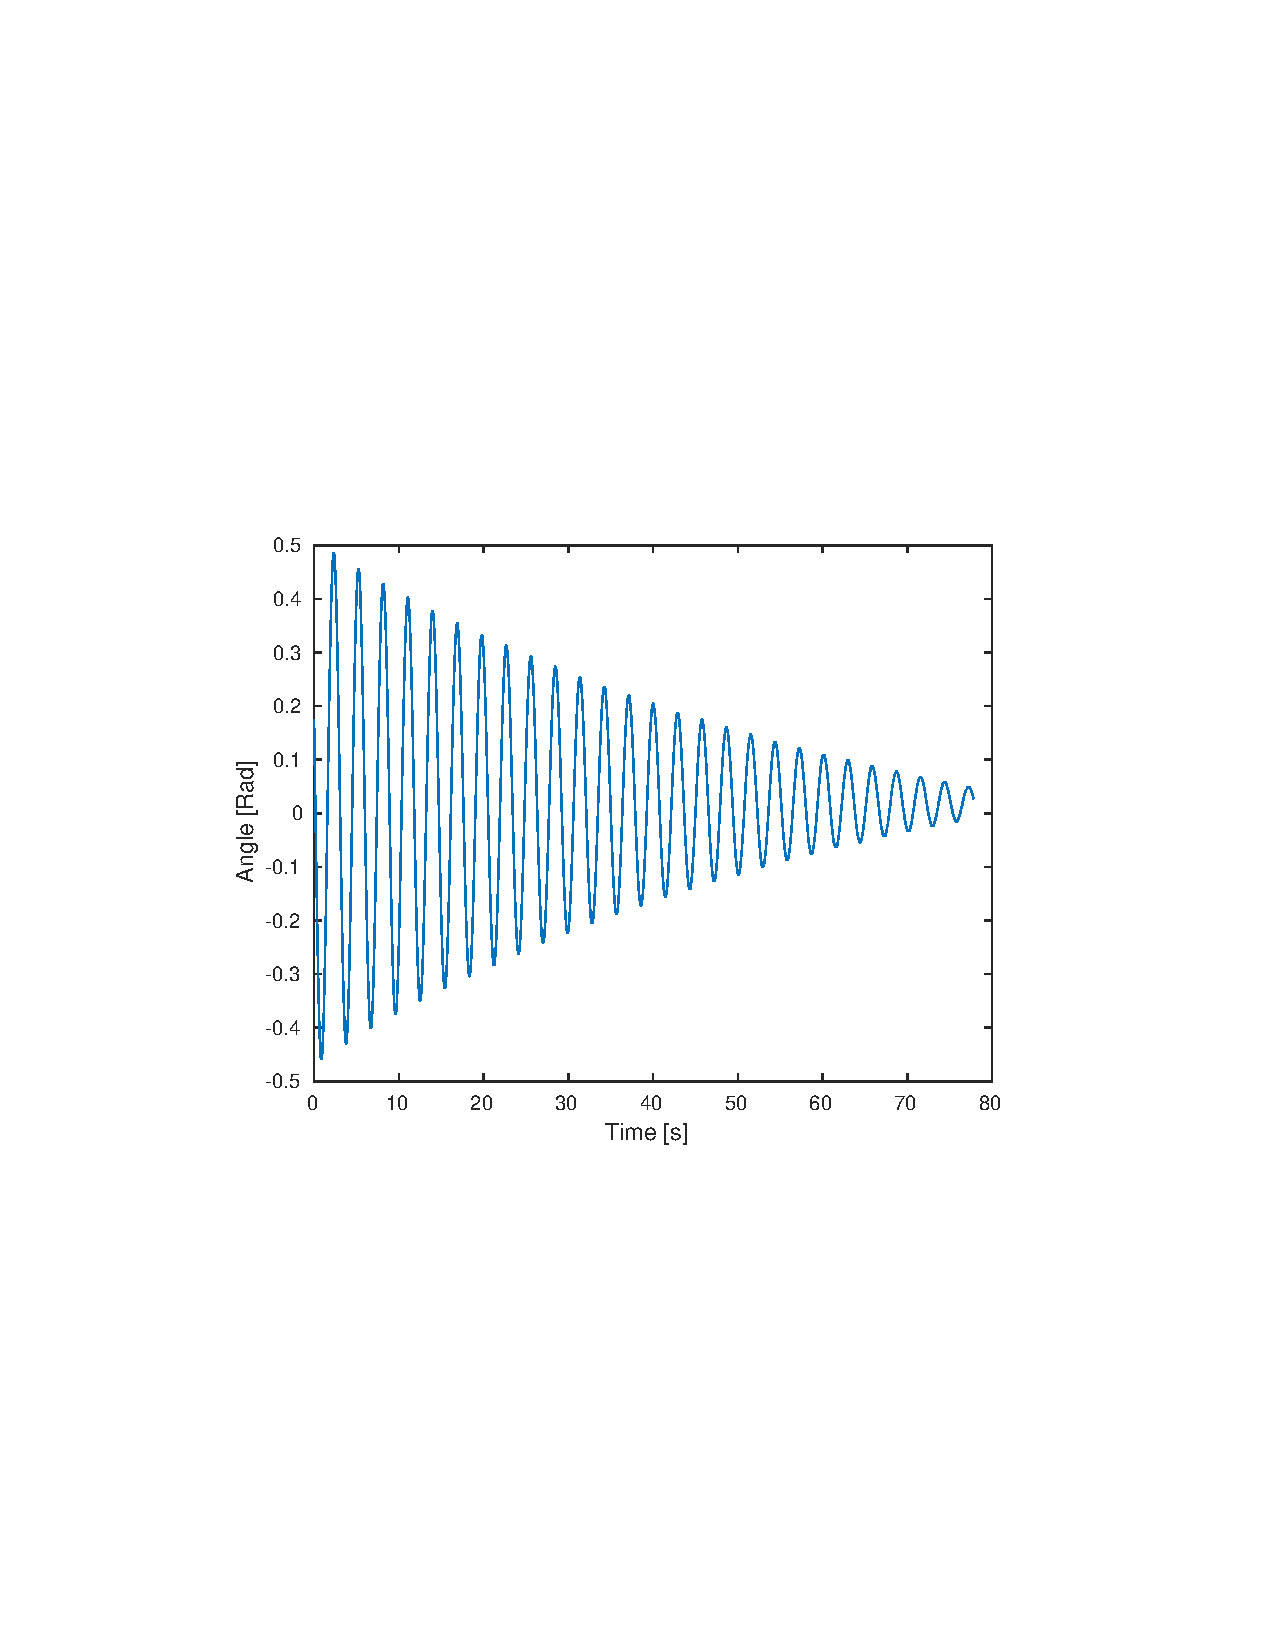
\includegraphics[width=14cm,trim=3cm 8.5cm 3cm 9cm,clip]
        {../res/img/sys11.pdf}
      \end{center}
      \caption{Dane pomiarowe drgań identyfikowanego wahadła}
      \label{plot:sys11}
    \end{figure}
    
    Wyznaczone parametry modelu zostały zestawione w tabeli \ref{tab:wyn11}.

    \begin{table}[!htb]
      \begin{center}
        \begin{tabular}{|c|c|}
          \hline
          $\omega_0$        & $ 2.1826 $ \\
          $\xi$             & $ 0.0125 $ \\
          $\alpha$          & $ 0.0181 $ \\
          $g$               & $ 1.1241\cdot 10^{-7} $ \\
          $x_{10}$          & $  0.1749 $ \\
          $x_{20}$          & $ -1.0718 $ \\
          $\sigma_{x}$      & $ 4.6571\cdot 10^{-4} $ \\
          $\sigma_{v}$      & $ 4.6571\cdot 10^{-4} $ \\
          \hline
          $\sigma_{\omega}$ & $ 2.4117\cdot 10^{-5} $ \\ 
          $\sigma_{\xi}$    & $ 4.3252\cdot 10^{-6} $ \\
          $\sigma_{x_{10}}$ & $ 0.0028 $ \\
          $\sigma_{x_{20}}$ & $ 0.0157 $ \\
          \hline
        \end{tabular}
      \end{center}
      \label{tab:wyn11}
      \caption{Wyniki identyfikacji}
    \end{table}
    
    \newpage
    
    Wynik dopasowania modelu do danych pomiarowych znajduje się na rysunku
    \ref{plot:est11}.

    \begin{figure}[!htb]
      \begin{center}
        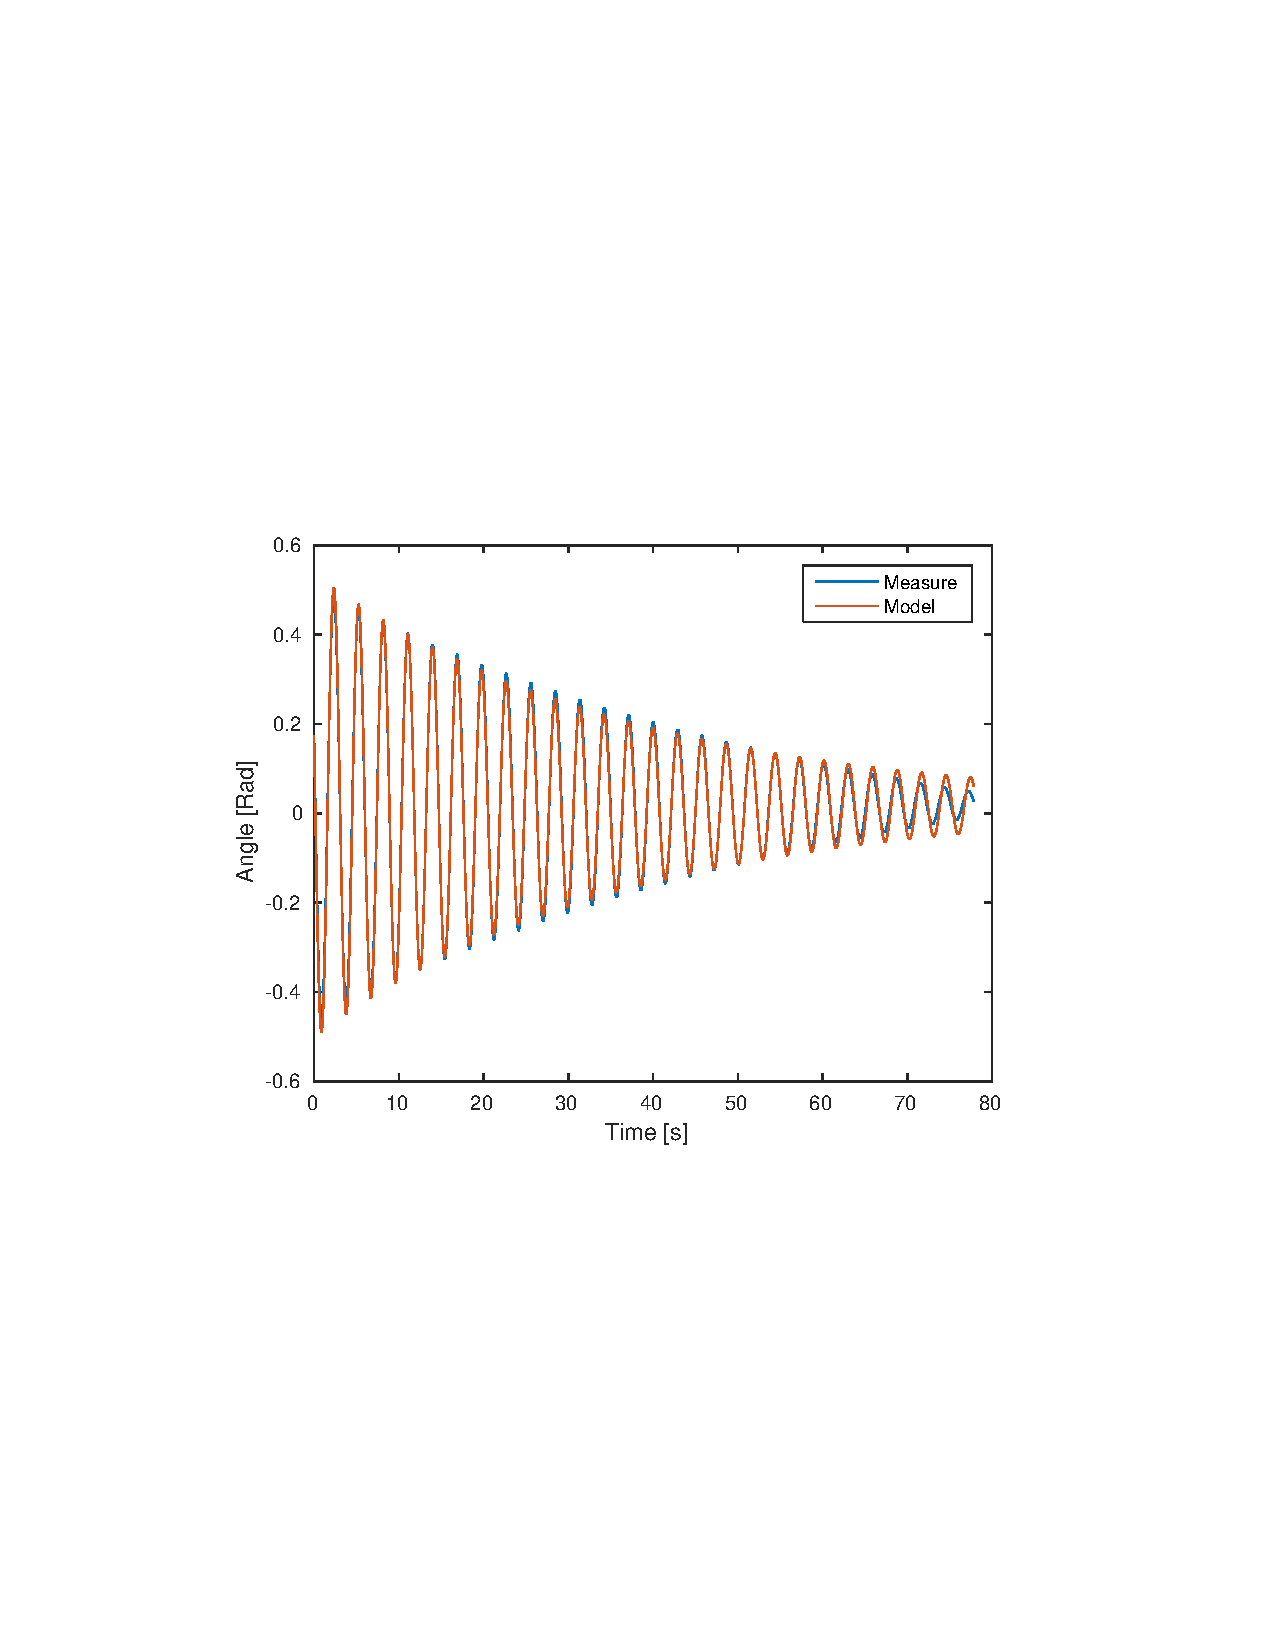
\includegraphics[width=14cm,trim=3cm 8.5cm 3cm 9cm,clip]
        {../res/img/est11.pdf}
      \end{center}
      \caption{Symulacja wahadła na tle jego rzeczywistej wartości}
      \label{plot:est11}
    \end{figure}
    
    Reszty modelu przedstawia rysunek \ref{plot:err11}.

    \begin{figure}[!htb]
      \begin{center}
        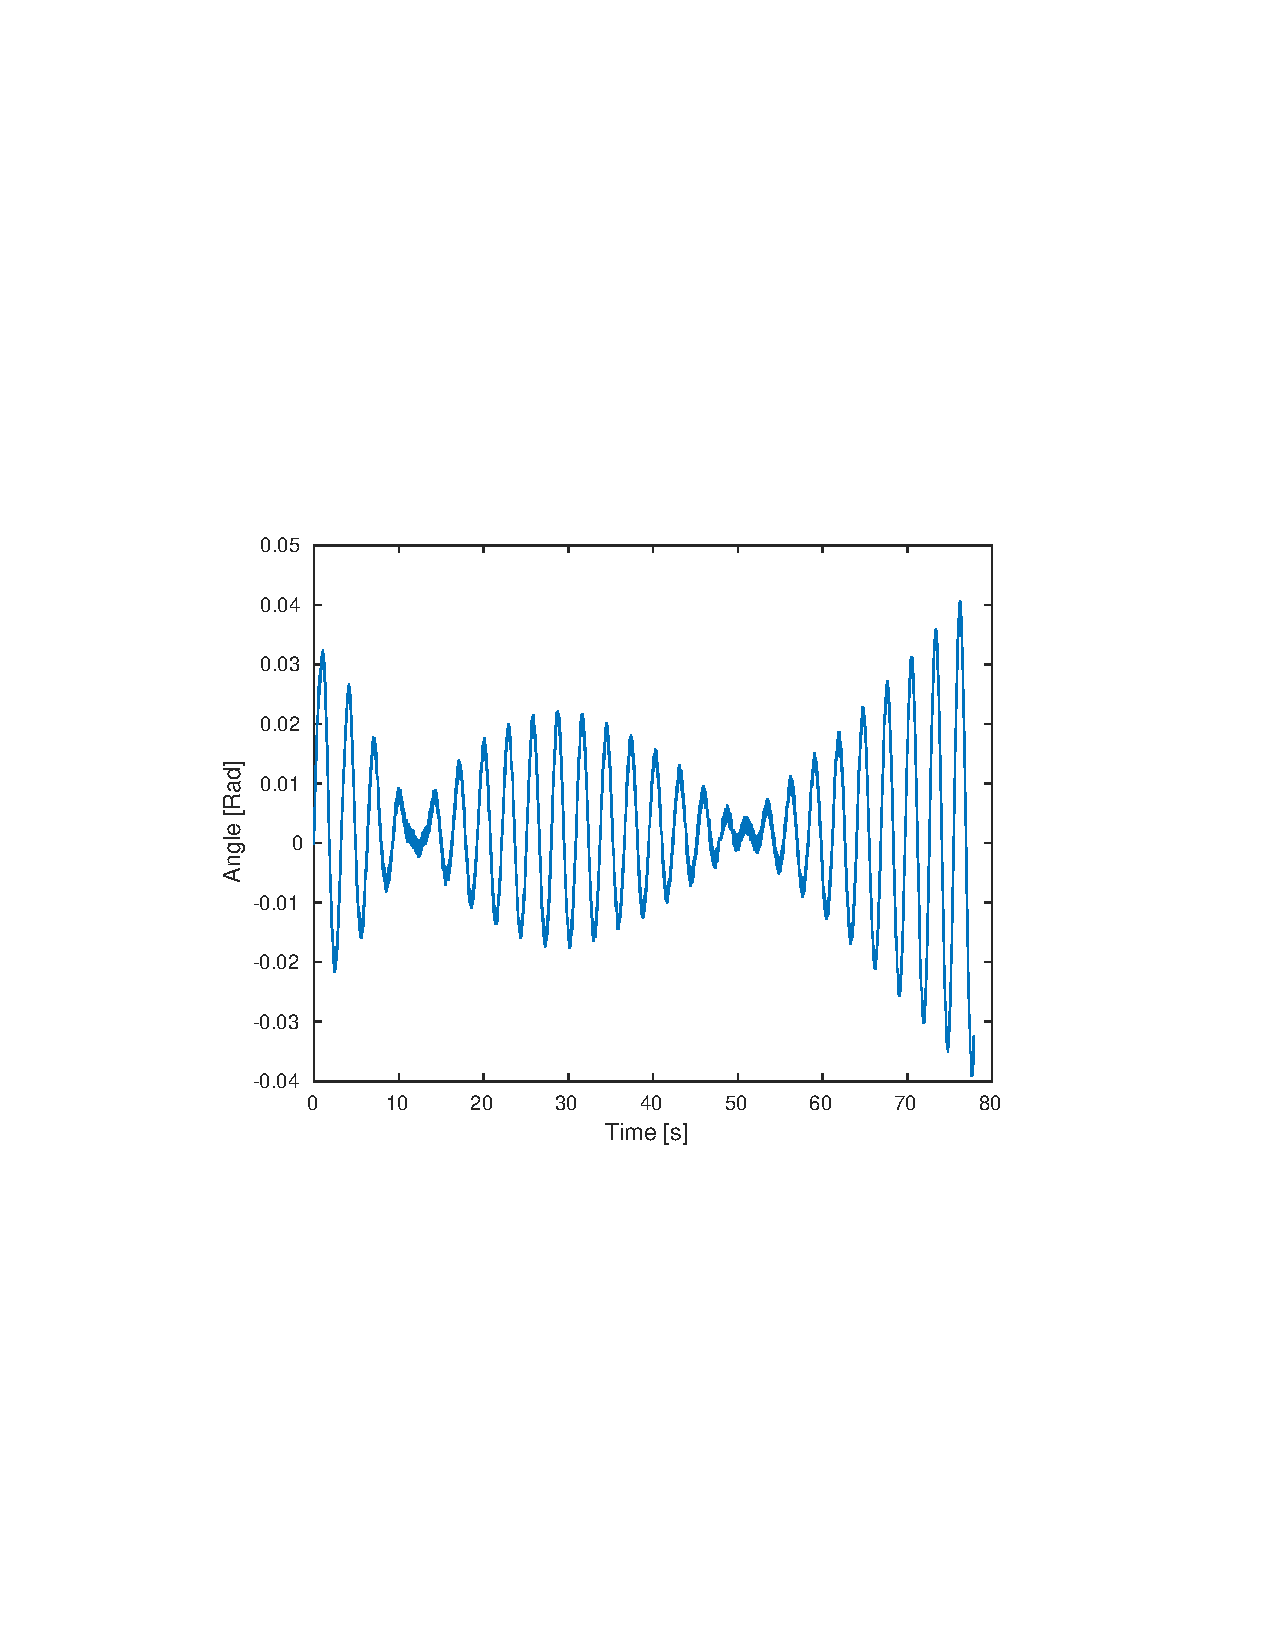
\includegraphics[width=14cm,trim=3cm 8.5cm 3cm 9cm,clip]
        {../res/img/err11.pdf}
      \end{center}
      \caption{Różnica realizacji modelu i danych pomiarowych}
      \label{plot:err11}
    \end{figure}
    
  \end{section}
    
  \newpage

  \begin{section}{Zadanie 2}
  
    Drugie zadanie miało identyczny przebieg jak zadanie pierwsze, z tą
    różnicą, iż do identyfikacji zostały użyte inne dane pomiarowe.
    
    Przebieg czasowy drgań identyfikowanego wahadła znajduje się na rysunku
    \ref{plot:sys12}.

    \begin{figure}[!htb]
      \begin{center}
        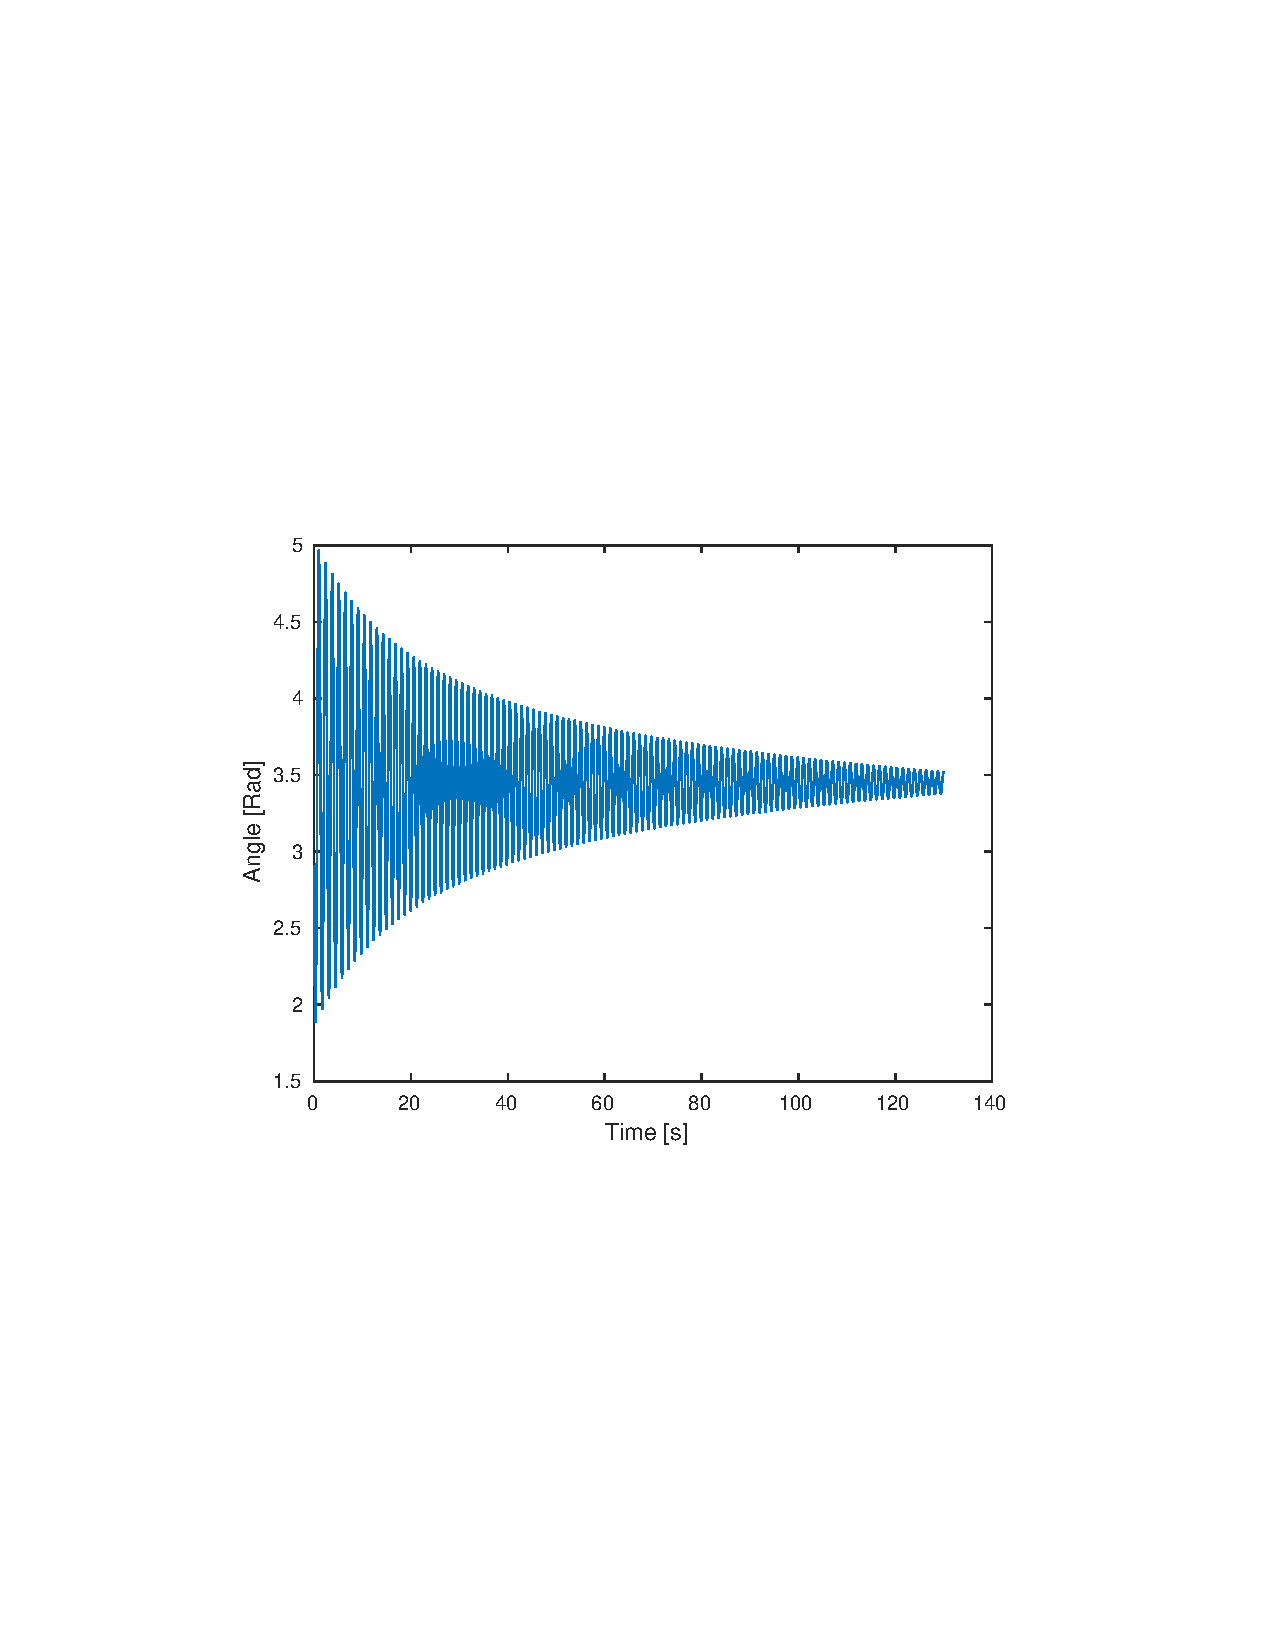
\includegraphics[width=14cm,trim=3cm 8.5cm 3cm 9cm,clip]
        {../res/img/sys12.pdf}
      \end{center}
      \caption{Dane pomiarowe drgań identyfikowanego wahadła}
      \label{plot:sys12}
    \end{figure}
    
    Wyznaczone parametry modelu zostały zestawione w tabeli \ref{tab:wyn12}.

    \begin{table}[!htb]
      \begin{center}
        \begin{tabular}{|c|c|}
          \hline
          $\omega_0$        & $ 5.2062 $ \\
          $\xi$             & $ 0.0049 $ \\
          $\alpha$          & $ 3.4499 $ \\
          $g$               & $ 7.9289\cdot 10^{-7} $ \\
          $x_{10}$          & $  3.0949 $ \\
          $x_{20}$          & $ -6.8040 $ \\
          $\sigma_{x}$      & $ 5.3271\cdot 10^{-4} $ \\
          $\sigma_{v}$      & $ 5.3271\cdot 10^{-4} $ \\
          \hline
          $\sigma_{\omega}$ & $ 4.7745\cdot 10^{-4} $ \\ 
          $\sigma_{\xi}$    & $ 6.1453\cdot 10^{-7} $ \\
          $\sigma_{x_{10}}$ & $ 0.2431 $ \\
          $\sigma_{x_{20}}$ & $ 0.3006 $ \\
          \hline
        \end{tabular}
      \end{center}
      \label{tab:wyn12}
      \caption{Wyniki identyfikacji}
    \end{table}
    
    \newpage
    
    Wynik dopasowania modelu do danych pomiarowych znajduje się na rysunku
    \ref{plot:est11}.

    \begin{figure}[!htb]
      \begin{center}
        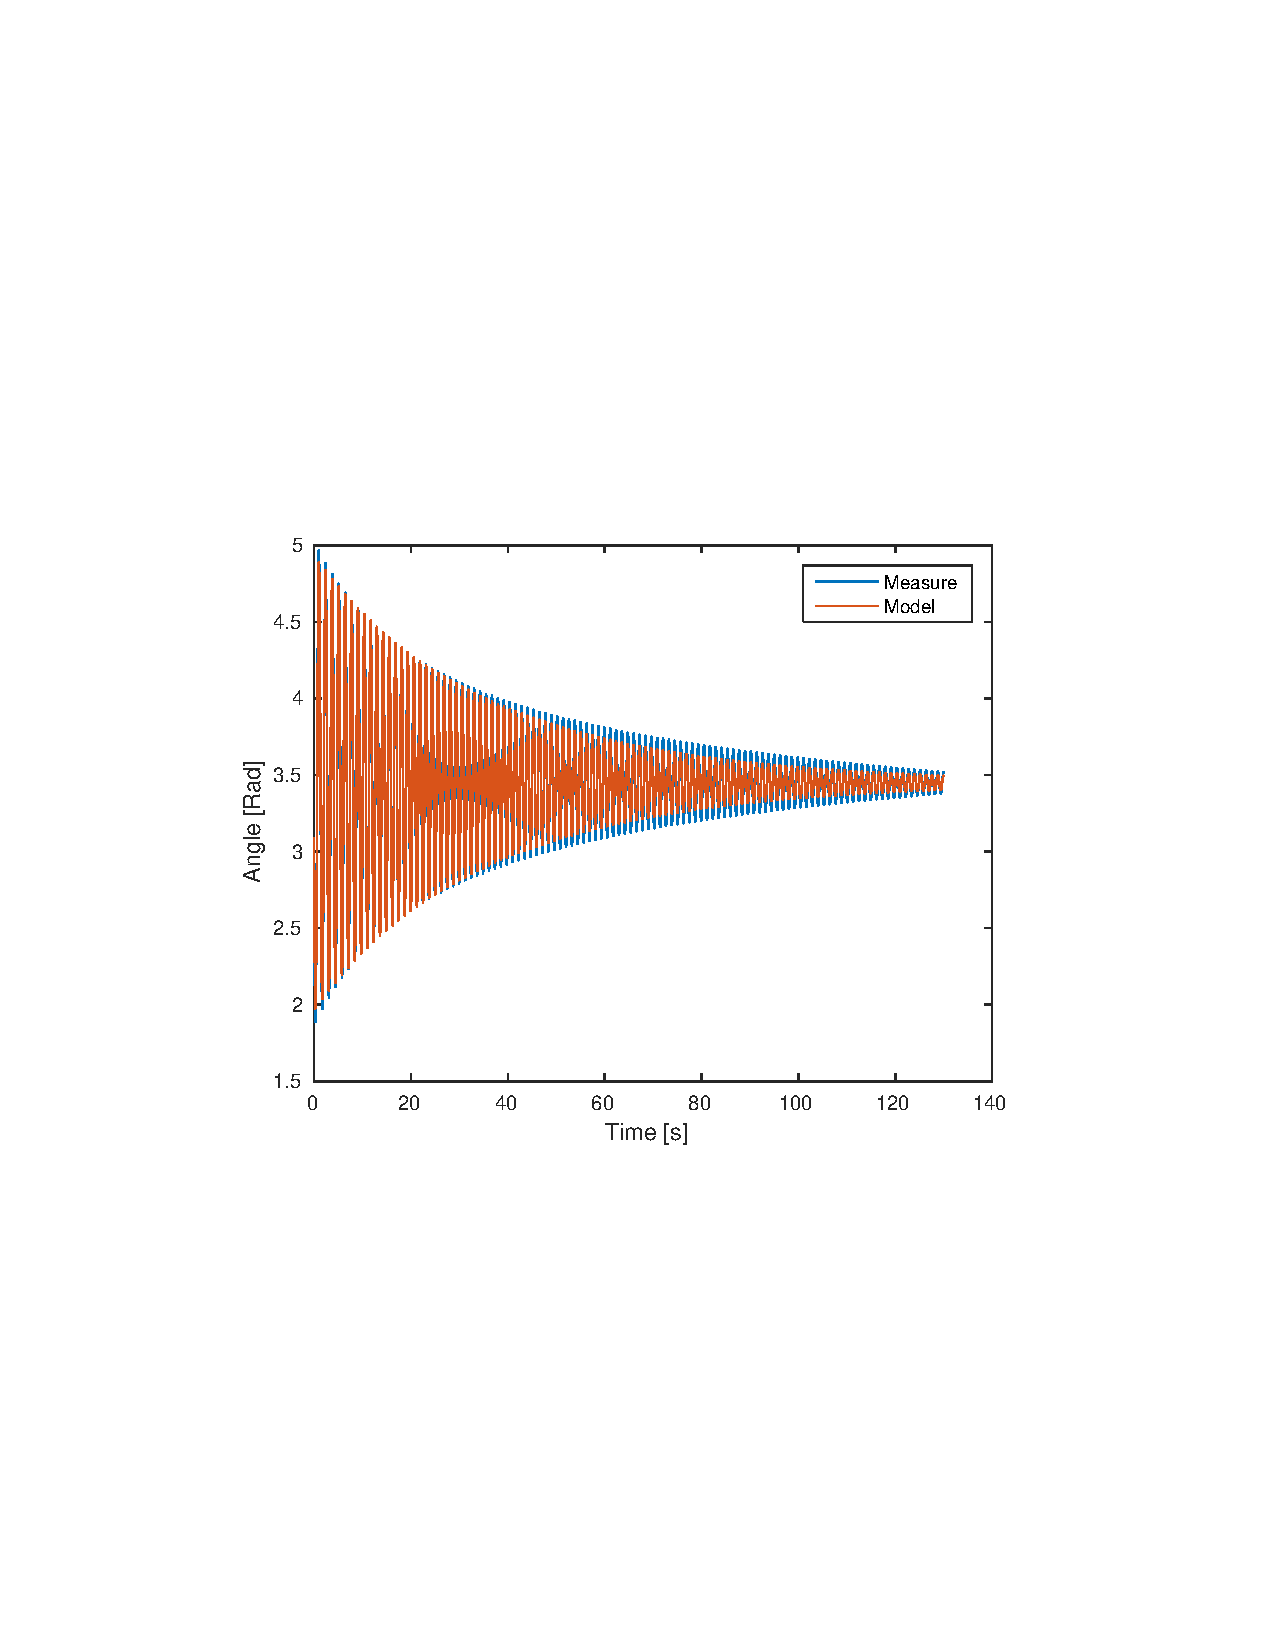
\includegraphics[width=14cm,trim=3cm 8.5cm 3cm 9cm,clip]
        {../res/img/est12.pdf}
      \end{center}
      \caption{Symulacja wahadła na tle jego rzeczywistej wartości}
      \label{plot:est12}
    \end{figure}
    
    Reszty modelu przedstawia rysunek \ref{plot:err12}.

    \begin{figure}[!htb]
      \begin{center}
        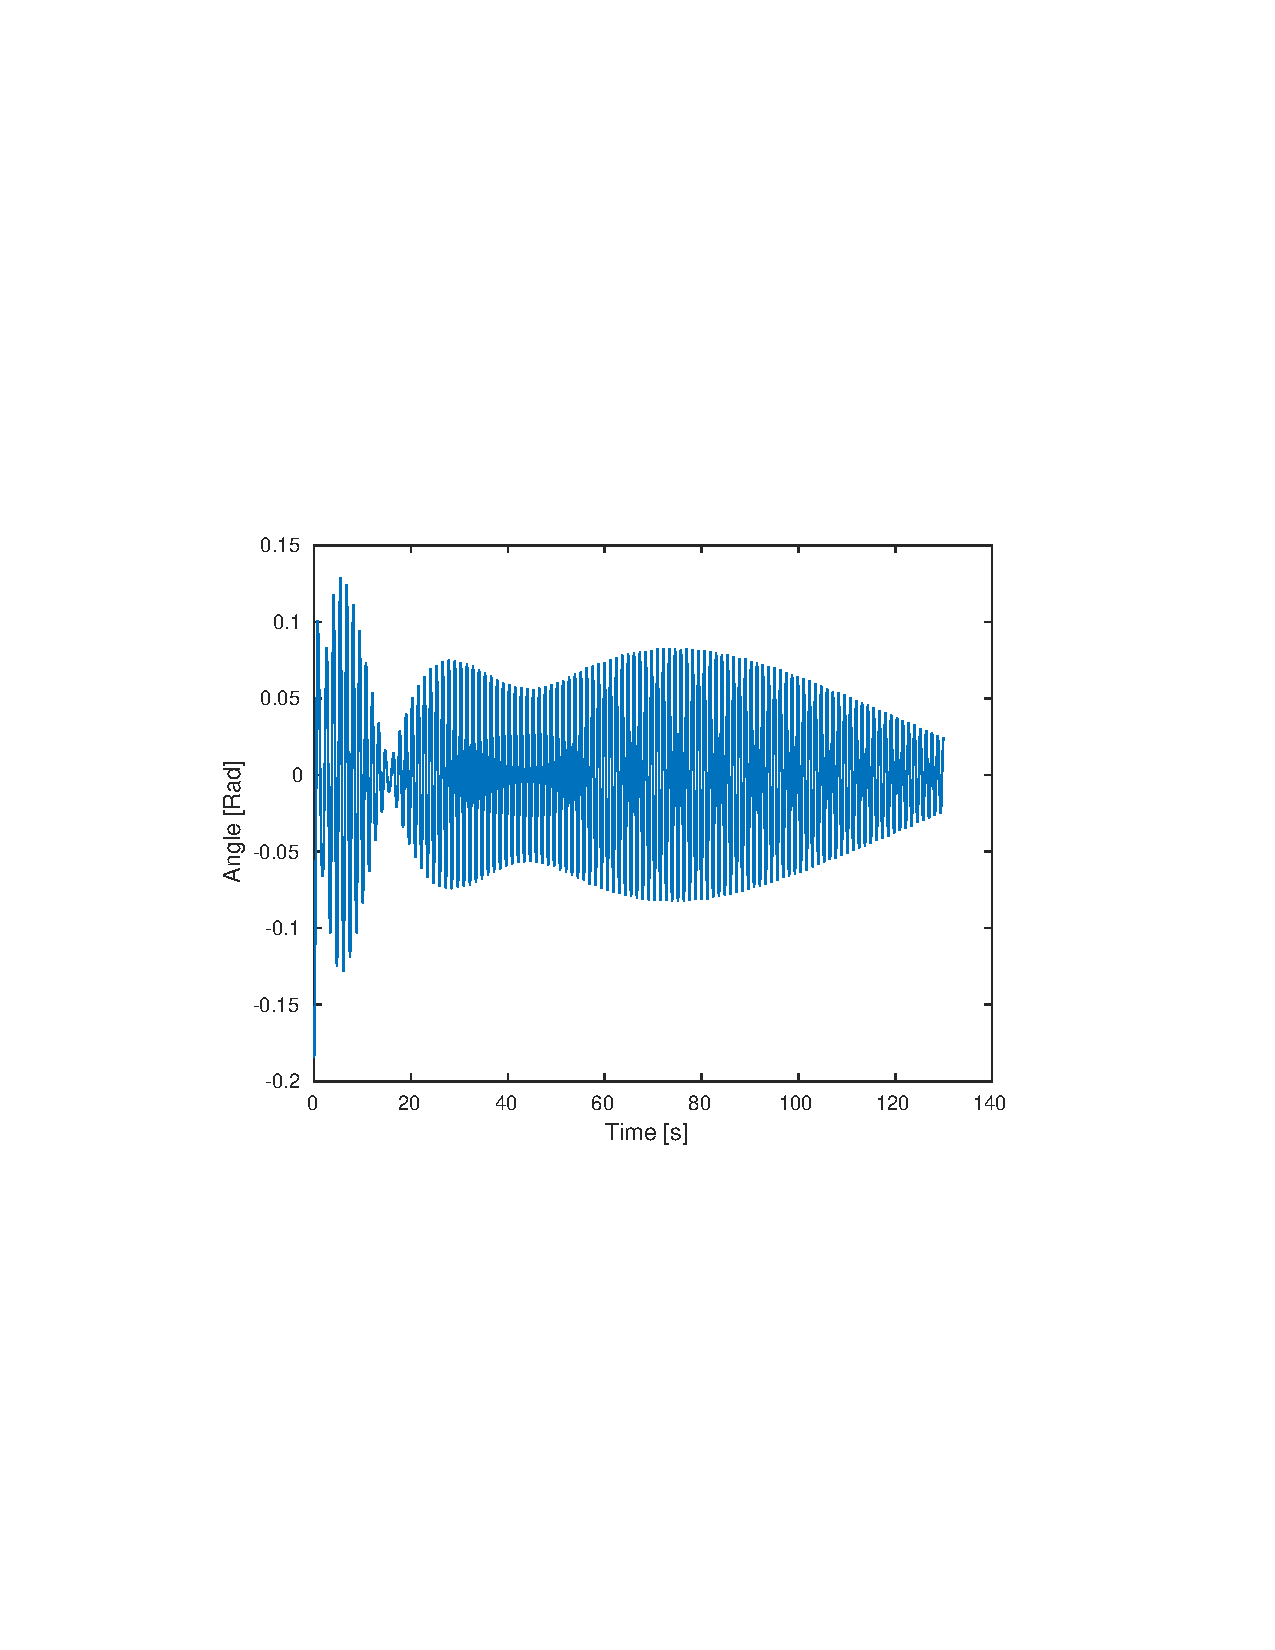
\includegraphics[width=14cm,trim=3cm 8.5cm 3cm 9cm,clip]
        {../res/img/err12.pdf}
      \end{center}
      \caption{Różnica realizacji modelu i danych pomiarowych}
      \label{plot:err12}
    \end{figure}
    
    \newpage

  \end{section}

  \begin{section}{Wnioski}
  
    W obydwu przypadkach identyfikowane parametry modelu nie pozwalały uzyskać
    dobrego dopasowania do danych pomiarowych. Zapewne zostało to spowodowane
    założeniem pewnego uproszczenia podczas wyprowadzania równań modelu.
    Obserwacja odpowiedzi modelu symulacyjnego na tle rzeczywistych danych
    pomiarowych sugeruje niezgodną z rzeczywistym zachowaniem metodę modelowania
    oporów ruchu.
    
    Celem weryfikacji tej hipotezy zostały zmodyfikowane równania modelu którego
    identyfikacja jest dokonywana. Nowe równania mają postać \ref{equ:sys1a}.
    
    \begin{equation}
      \begin{cases}
        dx_1=x_2dt \\
        dx_2=-\omega_0^2\sin(x_1-\alpha)dt-2\xi\omega\frac{x_2}{\sqrt{|x_2|}}dt+\sqrt{g}dw
      \end{cases}
      \label{equ:sys1a}
    \end{equation}
    \vspace{0.5cm}
    
    Wykonana została próba dla danych pomiarowych z zadania 1. Jak widać na
    rysunku \ref{plot:est11a}, dopasowanie modelu do danych symulacyjnych jest
    znacznie dokładniejsze niż w przypadku modelu \ref{equ:sys1}.

    \begin{figure}[!htb]
      \begin{center}
        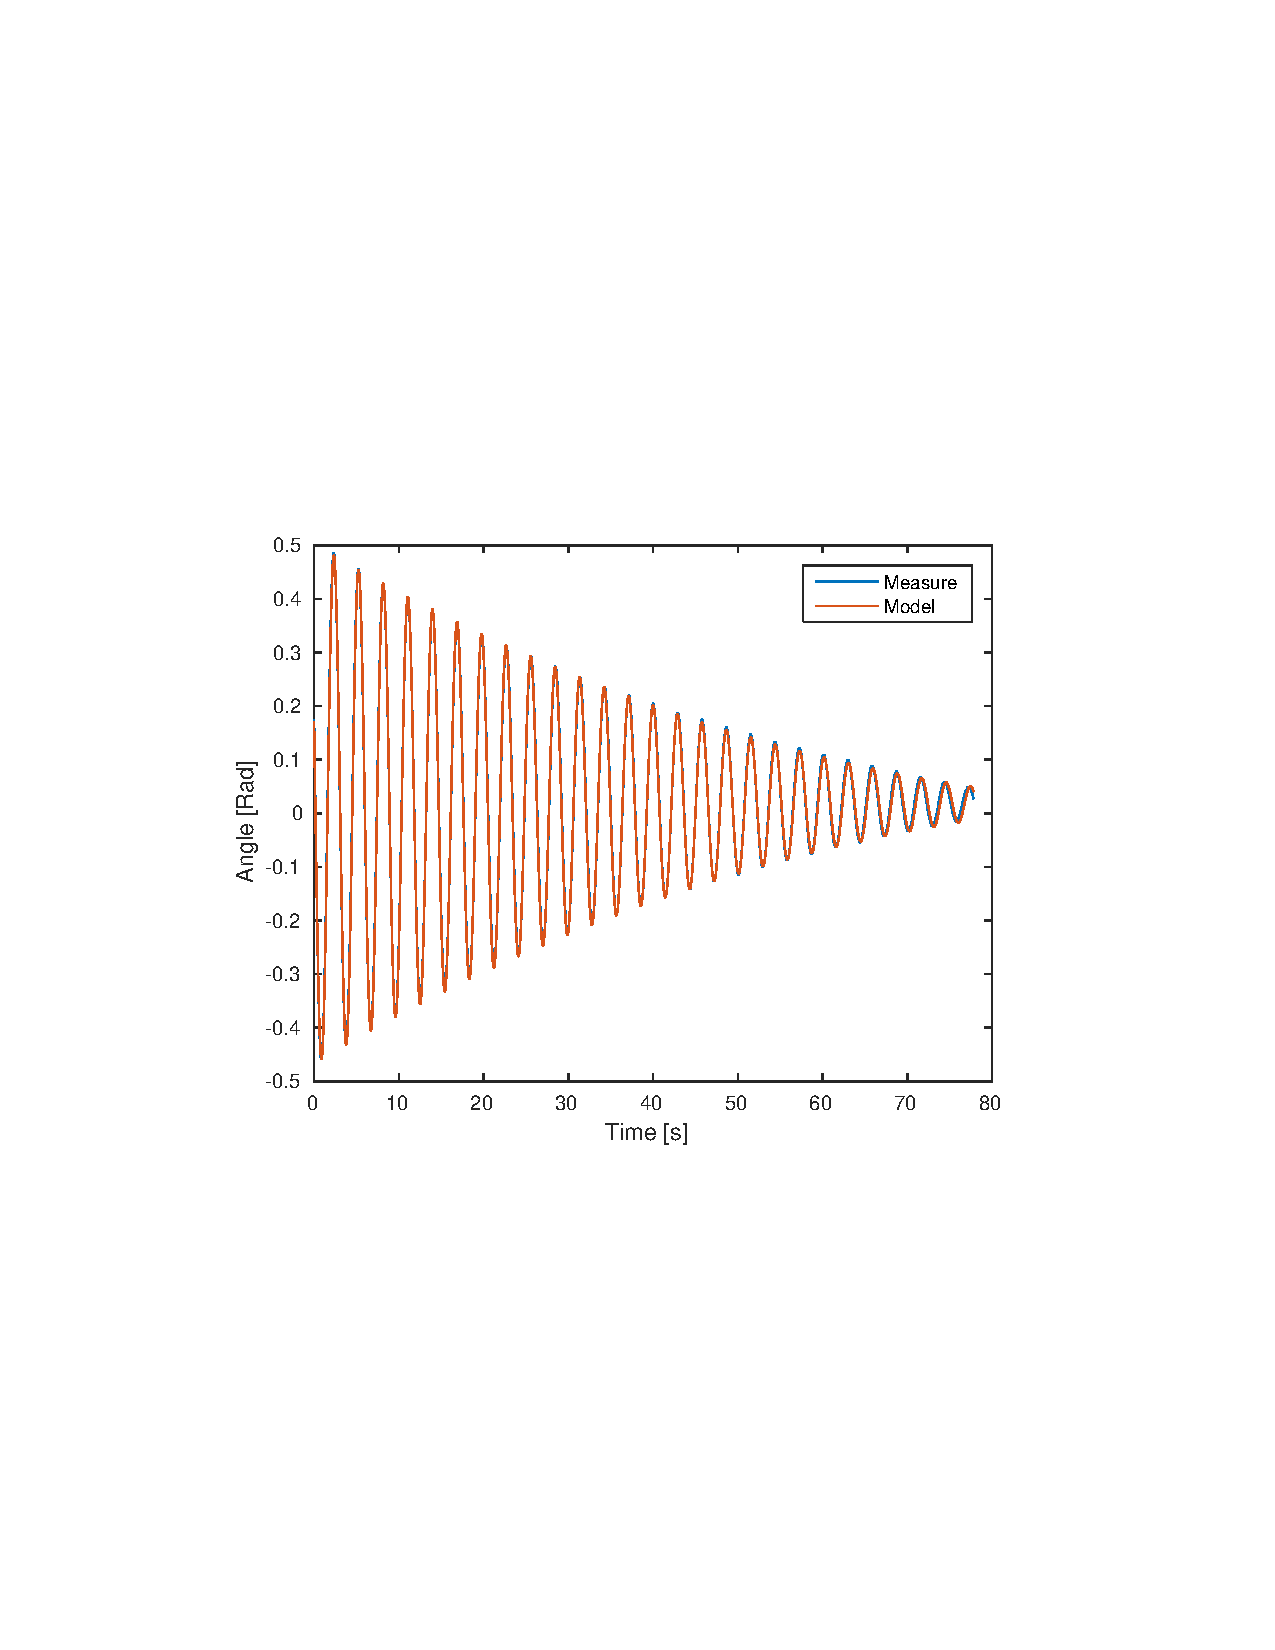
\includegraphics[width=14cm,trim=3cm 8.5cm 3cm 9cm,clip]
        {../res/img/est11a.pdf}
      \end{center}
      \caption{Symulacja wahadła na tle jego rzeczywistej wartości dla
      zmodyfikowanego modelu}
      \label{plot:est11a}
    \end{figure}
    
    Próby dopasowania z obydwu zadań generują reszty, nie będące szumem białym,
    co widać na rysunkach \ref{plot:err11} oraz \ref{plot:err12}, co za tym
    idzie nie przechodzą one testu $\chi^2$.
  
  \end{section}

\end{document}